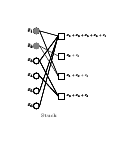
\begin{tikzpicture}
\def\horzgap{0.125in}; %Horizontal gap between nodes/levels
\def \gapVN{0.075in}; %vertical gap between nodes
\def \gapCN{0.1in}; %Horizontal gap between nodes


\def\nodewidth{0.5ex}; 
\def\nodewidthA{0.5ex};
\def \edgewidth{15ex}; 
\def\ext{0.1in};


\tikzstyle{check} = [rectangle, draw,line width=0.07mm, inner sep=0mm, minimum height=\nodewidthA, minimum width=\nodewidthA]
\tikzstyle{bit} = [circle, draw, line width=0.07mm, inner sep=0mm,  minimum size=\nodewidthA]
\tikzstyle{bituncover} = [circle, draw=none, line width=0.05mm, inner sep=0mm, fill=gray, minimum size=\nodewidthA]

 \def\moveX {1.8*\nodewidth};
\def\moveXA {2*\nodewidth};

            
\onslide<1>{             
\foreach \vn in {1,...,6}{
 \node[bit] (vn\vn) at (0,-\vn*\gapVN) {};
}

\foreach \vn in {1,...,6}{
\path (vn\vn) ++(-\nodewidth,0) node()[scale=0.25, inner sep=0mm] {\tiny{$\vec{x}_{\vn}$}};
}

\foreach \cn in {1,...,4}{
\node[check] (cn\cn) at (\horzgap,-\cn*\gapCN) {};
}

\draw[line width=0.05mm] (vn4.east)--(cn4.west);
\draw[line width=0.05mm] (vn3.east)--(cn4.west);

\draw[line width=0.05mm] (vn2.east)--(cn3.west);
\draw[line width=0.05mm] (vn1.east)--(cn3.west);

\draw[line width=0.05mm] (vn2.east)--(cn2.west);

\draw[line width=0.05mm] (vn1.east)--(cn1.west);
\draw[line width=0.05mm] (vn3.east)--(cn1.west);
\draw[line width=0.05mm] (vn5.east)--(cn1.west);
\draw[line width=0.05mm] (vn6.east)--(cn1.west);


\node [scale=0.2,anchor=west] at (cn1.east) {\tiny{$\vec{x}_1+\vec{x}_3+\vec{x}_5+\vec{x}_6+\vec{z}_1$}};
\node [scale=0.2,anchor=west] at (cn2.east) {\tiny{$\vec{x}_2+\vec{z}_2$}};
\node [scale=0.2,anchor=west] at (cn3.east) {\tiny{$\vec{x}_1+\vec{x}_2+\vec{z}_3$}};
\node [scale=0.2,anchor=west] at (cn4.east) {\tiny{$\vec{x}_3+\vec{x}_4+\vec{z}_4$}};

}

%-----------------------*(&^#@$^&*(^%$^&*(&^--------------------------------------------------------------------
%Dotted x_2
\onslide<2>{
\foreach \vn in {1,3,4,5,6}{
 \node[bit] (vn\vn) at (0,-\vn*\gapVN) {};
}

\foreach \vn in {1,3,4,5,6}{
\path (vn\vn) ++(-\nodewidth,0) node()[scale=0.25, inner sep=0mm] {\tiny{$\vec{x}_{\vn}$}};
}


\foreach \vn in {2}{
 \node[bituncover] (vn\vn) at (0,-\vn*\gapVN) {};
}

\foreach \vn in {2}{
\path (vn\vn) ++(-\nodewidth,0) node()[scale=0.25, inner sep=0mm] {\tiny{$\hat{\vec{x}}_2$}};
}


\foreach \cn in {1,...,4}{
\node[check] (cn\cn) at (\horzgap,-\cn*\gapCN) {};
}


\draw[line width=0.05mm] (vn4.east)--(cn4.west);
\draw[line width=0.05mm] (vn3.east)--(cn4.west);

\draw[line width=0.05mm, densely dotted] (vn2.east)--(cn3.west);
\draw[line width=0.05mm] (vn1.east)--(cn3.west);

\draw[line width=0.05mm, densely dotted] (vn2.east)--(cn2.west);

\draw[line width=0.05mm] (vn1.east)--(cn1.west);
\draw[line width=0.05mm] (vn3.east)--(cn1.west);
\draw[line width=0.05mm] (vn5.east)--(cn1.west);
\draw[line width=0.05mm] (vn6.east)--(cn1.west);

\node [scale=0.2,anchor=west] at (cn1.east) {\tiny{$\vec{x}_1+\vec{x}_3+\vec{x}_5+\vec{x}_6+\vec{z}_1$}};
\node [scale=0.2,anchor=west] at (cn2.east) {\tiny{$\vec{x}_2+\vec{z}_2$}};
\node [scale=0.2,anchor=west] at (cn3.east) {\tiny{$\vec{x}_1+\vec{x}_2+\vec{z}_3$}};
\node [scale=0.2,anchor=west] at (cn4.east) {\tiny{$\vec{x}_3+\vec{x}_4+\vec{z}_4$}};
}
%----------------------------------^%$#@%^&*()_*&^%$#^&*------------------------------------
%--Peeled x_2
\onslide<3>{
\foreach \vn in {1,3,4,5,6}{
 \node[bit] (vn\vn) at (0,-\vn*\gapVN) {};
}

\foreach \vn in {1,3,4,5,6}{
\path (vn\vn) ++(-\nodewidth,0) node()[scale=0.25, inner sep=0mm] {\tiny{$\vec{x}_{\vn}$}};
}


\foreach \vn in {2}{
 \node[bituncover] (vn\vn) at (0,-\vn*\gapVN) {};
}

\foreach \vn in {2}{
\path (vn\vn) ++(-\nodewidth,0) node()[scale=0.25, inner sep=0mm] {\tiny{$\hat{\vec{x}}_2$}};
}


\foreach \cn in {1,...,4}{
\node[check] (cn\cn) at (\horzgap,-\cn*\gapCN) {};
}


\draw[line width=0.05mm] (vn4.east)--(cn4.west);
\draw[line width=0.05mm] (vn3.east)--(cn4.west);

\draw[line width=0.05mm] (vn1.east)--(cn3.west);

\draw[line width=0.05mm] (vn1.east)--(cn1.west);
\draw[line width=0.05mm] (vn3.east)--(cn1.west);
\draw[line width=0.05mm] (vn5.east)--(cn1.west);
\draw[line width=0.05mm] (vn6.east)--(cn1.west);

\node [scale=0.2,anchor=west] at (cn1.east) {\tiny{$\vec{x}_1+\vec{x}_3+\vec{x}_5+\vec{x}_6+\vec{z}_1$}};
\node [scale=0.2,anchor=west] at (cn2.east) {\tiny{$\vec{z}_2$}};
\node [scale=0.2,anchor=west] at (cn3.east) {\tiny{$\vec{x}_1+\vec{z}_3$}};
\node [scale=0.2,anchor=west] at (cn4.east) {\tiny{$\vec{x}_3+\vec{x}_4+\vec{z}_4$}};
}

%---------%^&*^%$#^&----------------------------
%Dotted x_1
\onslide<4>{
\foreach \vn in {3,4,5,6}{
 \node[bit] (vn\vn) at (0,-\vn*\gapVN) {};
}

\foreach \vn in {1,2}{
 \node[bituncover] (vn\vn) at (0,-\vn*\gapVN) {};
}


\foreach \vn in {3,4,5,6}{
\path (vn\vn) ++(-\nodewidth,0) node()[scale=0.25, inner sep=0mm] {\tiny{$\vec{x}_{\vn}$}};
}

\foreach \vn in {1,2}{
\path (vn\vn) ++(-\nodewidth,0) node()[scale=0.25, inner sep=0mm] {\tiny{$\hat{\vec{x}}_{\vn}$}};
}

\foreach \cn in {1,...,4}{
\node[check] (cn\cn) at (\horzgap,-\cn*\gapCN) {};
}


\draw[line width=0.05mm] (vn4.east)--(cn4.west);
\draw[line width=0.05mm] (vn3.east)--(cn4.west);

\draw[line width=0.05mm, densely dotted] (vn1.east)--(cn3.west);
\draw[line width=0.05mm, densely dotted] (vn1.east)--(cn1.west);

\draw[line width=0.05mm] (vn3.east)--(cn1.west);
\draw[line width=0.05mm] (vn5.east)--(cn1.west);
\draw[line width=0.05mm] (vn6.east)--(cn1.west);


\node [scale=0.2,anchor=west] at (cn1.east) {\tiny{$\vec{x}_1+\vec{x}_3+\vec{x}_5+\vec{x}_6+\vec{z}_1$}};
\node [scale=0.2,anchor=west] at (cn2.east) {\tiny{$\vec{z}_2$}};
\node [scale=0.2,anchor=west] at (cn3.east) {\tiny{$\vec{x}_1+\vec{z}_3$}};
\node [scale=0.2,anchor=west] at (cn4.east) {\tiny{$\vec{x}_3+\vec{x}_4+\vec{z}_4$}};
}

%----------------------------------^%$#@%^&*()_*&^%$#^&*------------------------------------
%-peeled off x_1
\onslide<5>{
\foreach \vn in {3,4,5,6}{
 \node[bit] (vn\vn) at (0,-\vn*\gapVN) {};
}

\foreach \vn in {1,2}{
 \node[bituncover] (vn\vn) at (0,-\vn*\gapVN) {};
}


\foreach \vn in {3,4,5,6}{
\path (vn\vn) ++(-\nodewidth,0) node()[scale=0.25, inner sep=0mm] {\tiny{$\vec{x}_{\vn}$}};
}

\foreach \vn in {1,2}{
\path (vn\vn) ++(-\nodewidth,0) node()[scale=0.25, inner sep=0mm] {\tiny{$\hat{\vec{x}}_{\vn}$}};
}

\foreach \cn in {1,...,4}{
\node[check] (cn\cn) at (\horzgap,-\cn*\gapCN) {};
}


\draw[line width=0.05mm] (vn4.east)--(cn4.west);
\draw[line width=0.05mm] (vn3.east)--(cn4.west);

\draw[line width=0.05mm] (vn3.east)--(cn1.west);
\draw[line width=0.05mm] (vn5.east)--(cn1.west);
\draw[line width=0.05mm] (vn6.east)--(cn1.west);


\node [scale=0.2,anchor=west] at (cn1.east) {\tiny{$\vec{x}_3+\vec{x}_5+\vec{x}_6+\vec{z}_1$}};
\node [scale=0.2,anchor=west] at (cn2.east) {\tiny{$\vec{z}_2$}};
\node [scale=0.2,anchor=west] at (cn3.east) {\tiny{$\vec{z}_3$}};
\node [scale=0.2,anchor=west] at (cn4.east) {\tiny{$\vec{x}_3+\vec{x}_4+\vec{z}_4$}};
}

%----------------------------------^%$#@%^&*()_*&^%$#^&*------------------------------------
\onslide<6>{
\foreach \vn in {3,4,5,6}{
 \node[bit] (vn\vn) at (0,-\vn*\gapVN) {};
}

\foreach \vn in {1,2}{
 \node[bituncover] (vn\vn) at (0,-\vn*\gapVN) {};
}


\foreach \vn in {3,4,5,6}{
\path (vn\vn) ++(-\nodewidth,0) node()[scale=0.25, inner sep=0mm] {\tiny{$\vec{x}_{\vn}$}};
}

\foreach \vn in {1,2}{
\path (vn\vn) ++(-\nodewidth,0) node()[scale=0.25, inner sep=0mm] {\tiny{$\hat{\vec{x}}_{\vn}$}};
}

\foreach \cn in {1,...,4}{
\node[check] (cn\cn) at (\horzgap,-\cn*\gapCN) {};
}


\draw[line width=0.05mm] (vn4.east)--(cn4.west);
\draw[line width=0.05mm] (vn3.east)--(cn4.west);

\draw[line width=0.05mm] (vn3.east)--(cn1.west);
\draw[line width=0.05mm] (vn5.east)--(cn1.west);
\draw[line width=0.05mm] (vn6.east)--(cn1.west);


\node [scale=0.2,anchor=west] at (cn1.east) {\tiny{$\vec{x}_3+\vec{x}_5+\vec{x}_6+\vec{z}_1$}};
\node [scale=0.2,anchor=west] at (cn2.east) {\tiny{$\vec{z}_2$}};
\node [scale=0.2,anchor=west] at (cn3.east) {\tiny{$\vec{z}_3$}};
\node [scale=0.2,anchor=west] at (cn4.east) {\tiny{$\vec{x}_3+\vec{x}_4+\vec{z}_4$}};

\node[scale=0.35] () at (0.5*\horzgap,-5*\gapCN) {\tiny{Stuck}};
}
\end{tikzpicture}